\documentclass[12pt]{article}
\usepackage[utf8]{inputenc}
\usepackage[T1]{fontenc}
\usepackage{unicode-math}
\newcommand{\EE}{\mathbb{E}}
\newcommand{\R}{\mathbb{R}}
\usepackage{amsmath,amsfonts,amssymb}
\usepackage{graphicx}
\usepackage{a4wide}
\usepackage[backend=biber,style=numeric,sorting=none]{biblatex}
\usepackage{import}
%\bibliographystyle{unsrt}
\addbibresource{draft.bib}

% Comments for co-authors (optional)
\newcommand{\coauthorcomment}[2]{{\color{#1} \textbf{#2}}}

% Title and author information
% \usepackage[pagebackref=true]{hyperref}  % hyperlinks
% \renewcommand*{\backrefalt}[4]{%
%     \ifcase #1 \footnotesize{(Not cited.)}%
%     \or        \footnotesize{(Cited on page~#2)}%
%     \else      \footnotesize{(Cited on pages~#2)}%
%     \fi}
% simple URL typesetting
\usepackage{booktabs}       % professional-quality tables
\usepackage{amsfonts}       % blackboard math symbols
\usepackage{nicefrac}       % compact symbols for 1/2, etc.
\usepackage{microtype}      % microtypography
%\usepackage{slashbox,pict2e}
\usepackage{comment}
\usepackage{amssymb, amsmath, latexsym}
% \usepackage{fullpage}
\usepackage{url}

\usepackage{algorithm}
\usepackage{algorithmic}
% \usepackage{algpseudocode}


\usepackage{tabularx}
\usepackage{paralist}
\usepackage{mathtools}
%\usepackage{tcolorbox}
%\usepackage{xcolor}

\usepackage{bbm} %for indicators 1
\usepackage{wrapfig}
\usepackage{makecell}
\usepackage{multirow}
\usepackage{booktabs}

\usepackage{nicefrac}       % nice fractions

\usepackage{boxhandler}
\usepackage[flushleft]{threeparttable} % http://ctan.org/pkg/threeparttable

\usepackage{caption}
\usepackage{multirow}
\usepackage{colortbl}
\definecolor{bgcolor}{rgb}{0.8,1,1}
\definecolor{bgcolor2}{rgb}{0.8,1,0.8}
\definecolor{niceblue}{rgb}{0.0,0.19,0.56}

\usepackage{hyperref}
\hypersetup{colorlinks,linkcolor={blue},citecolor={niceblue},urlcolor={blue}}

% \usepackage{natbib}
% \bibliographystyle{abbrvnat}
% \usepackage{sidecap}
% \renewcommand{\bibname}{References}
% \renewcommand{\bibsection}{\subsubsection*{\bibname}}
%\bibliographystyle{plain}


\renewcommand{\algorithmicrequire}{\textbf{Input:}}
\renewcommand{\algorithmicensure}{\textbf{Output:}}

% \usepackage[dvipsnames]{xcolor}
\usepackage{pifont}
\definecolor{PineGreen}{RGB}{0,110,51}
\definecolor{BrickRed}{RGB}{143,20,2}
\newcommand{\cmark}{{\color{PineGreen}\ding{51}}}%
\newcommand{\xmark}{{\color{BrickRed}\ding{55}}}%


\usepackage{tikz-cd} %for a diagram

\DeclareMathOperator*{\argmax}{arg\,max}
\DeclareMathOperator*{\argmin}{arg\,min}
% \usepackage{subfigure} 
\newcommand{\Exp}{\mathbf{E}}
\newcommand{\Prob}{\mathbf{P}}
\newcommand{\R}{\mathbb{R}}
\newcommand{\eqdef}{\stackrel{\text{def}}{=}}
\newcommand{\ve}[2]{\left\langle #1 , #2 \right\rangle}
\def\<#1,#2>{\left\langle #1,#2\right\rangle}

\newcommand{\oldstuff}[1]{ {\small \color{blue} #1}}
\newcommand{\redstuff}[1]{ {\small \color{red} #1}}

% for even table widths
\newcolumntype{Y}{>{\centering\arraybackslash}X}


\usepackage{xspace}

% Define the figure size
\newcommand\figscale{0.25}
\newcommand\evofigscale{0.21}


%\newcommand{\squeeze}{\textstyle} % when deployed
\newcommand{\squeeze}{} % when not deployed

\newcommand{\algname}[1]{{\sf  #1}\xspace}
\newcommand{\algnamex}[1]{{\sf #1}\xspace}

\newcommand\tagthis{\addtocounter{equation}{1}\tag{\theequation}}

\newcommand{\circledOne}{\text{\ding{172}}}
\newcommand{\circledTwo}{\text{\ding{173}}}
\newcommand{\circledThree}{\text{\ding{174}}}
\newcommand{\circledFour}{\text{\ding{175}}}
\newcommand{\circledFive}{\text{\ding{176}}}
\newcommand{\circledSix}{\text{\ding{177}}}
\newcommand{\circledSeven}{\text{\ding{178}}}
\newcommand{\circledEight}{\text{\ding{179}}}
\newcommand{\circledNine}{\text{\ding{180}}}
\newcommand{\circledTen}{\text{\ding{181}}}
\newcommand{\qed}{\hfill\blacksquare}
% TO DO NOTES 
\usepackage[colorinlistoftodos,bordercolor=orange,backgroundcolor=orange!20,linecolor=orange,textsize=scriptsize]{todonotes}

\newcommand{\alexander}[1]{\todo[inline]{{\textbf{Alexander:} \emph{#1}}}}
\newcommand{\eduard}[1]{\todo[inline]{{\textbf{Eduard:} \emph{#1}}}}
\newcommand{\nikita}[1]{\todo[inline]{{\textbf{Nikita:} \emph{#1}}}}
\newcommand{\Aleksandr}[1]{\todo[inline]{{\textbf{Aleksandr:} \emph{#1}}}}



\renewcommand{\Re}{\mathrm{Re}}
\renewcommand{\Im}{\mathrm{Im}}
\newcommand{\Sp}{\mathrm{Sp}}
\newcommand{\Id}{\mathrm{Id}}

\newcommand{\Tr}{\mathrm{Tr}}
\newcommand{\KL}{\mathrm{KL}}

% caligraphic
\newcommand{\cA}{{\cal A}}
\newcommand{\cB}{{\cal B}}
\newcommand{\cC}{{\cal C}}
\newcommand{\cD}{{\cal D}}
\newcommand{\cE}{{\cal E}}
\newcommand{\cF}{{\cal F}}
\newcommand{\cG}{{\cal G}}
\newcommand{\cH}{{\cal H}}
\newcommand{\cJ}{{\cal J}}
\newcommand{\cK}{{\cal K}}
\newcommand{\cL}{{\cal L}}
\newcommand{\cM}{{\cal M}}
\newcommand{\cN}{{\cal N}}
\newcommand{\cO}{{\cal O}}
\newcommand{\cP}{{\cal P}}
\newcommand{\cQ}{{\cal Q}}
\newcommand{\cR}{{\cal R}}
\newcommand{\cS}{{\cal S}}
\newcommand{\cT}{{\cal T}}
\newcommand{\cU}{{\cal U}}
\newcommand{\cV}{{\cal V}}
\newcommand{\cX}{{\cal X}}
\newcommand{\cY}{{\cal Y}}
\newcommand{\cW}{{\cal W}}
\newcommand{\cZ}{{\cal Z}}
\newcommand{\Var}{\mathrm{Var}}

% matrices
\newcommand{\mA}{{\bf A}}
\newcommand{\mB}{{\bf B}}
\newcommand{\mC}{{\bf C}}
\newcommand{\mE}{{\bf E}}
\newcommand{\mF}{{\bf F}}
\newcommand{\mG}{{\bf G}}
\newcommand{\mH}{{\bf H}}
\newcommand{\mI}{{\bf I}}
\newcommand{\mJ}{{\bf J}}
\newcommand{\mK}{{\bf K}}
\newcommand{\mL}{{\bf L}}
\newcommand{\mM}{{\bf M}}
\newcommand{\mN}{{\bf N}}
\newcommand{\mO}{{\bf O}}
\newcommand{\mP}{{\bf P}}
\newcommand{\mQ}{{\bf Q}}
\newcommand{\mR}{{\bf R}}
\newcommand{\mS}{{\bf S}}
\newcommand{\mT}{{\bf T}}
\newcommand{\mU}{{\bf U}}
\newcommand{\mV}{{\bf V}}
\newcommand{\mW}{{\bf W}}
\newcommand{\mX}{{\bf X}}
\newcommand{\mY}{{\bf Y}}
\newcommand{\mZ}{{\bf Z}}

\newcommand{\sign}{\mathrm{sign}}
\newcommand{\cnorm}{x}
\newcommand{\EE}{\mathbb{E}}
\newcommand{\PP}{\mathbb{P}}
\newcommand{\CC}{\mathbb{C}}
\newcommand{\VV}{\mathbf{V}}

\newcommand{\prox}{\mathop{\mathrm{prox}}\nolimits}


\newcommand{\proxR}{\prox_{\gamma R}}
\newcommand{\proxkR}{\prox_{\gamma^k R}}
\newcommand{\mean}{\overline}
\newcommand{\sumin}{\sum_{i=1}^n}

\newcommand{\tx}{\widetilde{x}}
\newcommand{\tX}{\widetilde{X}}
\newcommand{\ty}{\widetilde{y}}
\newcommand{\tF}{\widetilde{F}}

\newcommand{\tnabla}{\widetilde{\nabla}}


\newcommand{\hx}{\widehat{x}}
\newcommand{\hy}{\widehat{y}}


\def\Bxi{\boldsymbol{\xi}}

\def\clip{\texttt{clip}}
\def\avg{\texttt{avg}}
\def\gap{\texttt{Gap}}



\usepackage{hyperref}
\graphicspath{{plots/}}

\usepackage{makecell}

\usepackage{accents}
\newlength{\dhatheight}
\newcommand{\doublehat}[1]{%
    \settoheight{\dhatheight}{\ensuremath{\hat{#1}}}%
    \addtolength{\dhatheight}{-0.35ex}%
    \hat{\vphantom{\rule{1pt}{\dhatheight}}%
    \smash{\hat{#1}}}}


\usepackage{pgfplotstable} % loads pgfplots which loads tikz
\usetikzlibrary{automata, positioning, arrows, shapes, fit, calc, intersections}
\usepgfplotslibrary{statistics}

\newcommand{\dotprod}[2]{\langle #1,#2 \rangle} % Скалярное произведение




\def\la{\langle}
\def\ra{\rangle}
\usepackage{enumitem}
\usepackage{algorithm}
\usepackage{algorithmic}
\usepackage{algpseudocode}
\usepackage{subcaption}
\usepackage{graphicx}
\usepackage{amsthm}
\newtheorem{assumption}{Assumption}
\newtheorem{lemma}{Lemma}
\newtheorem{proposition}{Proposition}
\newtheorem{theorem}{Theorem}
\newtheorem{corollary}{Corollary}
\newtheorem{definition}{Definition}
\newtheorem{remark}{Remark}
\usepackage{subfigure}

\title{Sign operator for $(L_0, L_1)$-smooth optimization}

\author{
  Mark Ikonnikov\\
  \texttt{ikonnikov.mi@phystech.edu}
  \and
  Nikita Kornilov\\
  \texttt{kornilov.nm@phystech.edu}
}

\date{\today}

\begin{document}
\maketitle

\begin{abstract}
In Machine Learning, the non-smoothness of optimization problems, the high cost of communicating gradients between workers, and severely corrupted data during training necessitate further research of optimization methods under broader assumptions. This paper explores the efficacy of sign-based methods, which address slow transmission by communicating only the sign of each stochastic gradient. We investigate these methods for $(L_0, L_1)$-smooth problems, which encompass a wider range of problems than the $L$-smoothness assumption. To address the problem of data accuracy, we introduce the convergence bounds for \textit{$(L_0, L_1)$ SignSGD} and \textit{M-SignSGD} under heavy-tailed noise, defined as noise with bounded $\kappa$-th moment $\kappa \in (1,2]$.
\end{abstract}

\paragraph{Keywords:} Sign-based methods, $(L_0, L_1)$-smoothness, high-probability convergence, heavy-tailed noise.

\paragraph{ Highlights below to be fixed later (these are our hopes for the paper)}

\paragraph{ Highlights:}
\begin{enumerate}
\item Proves convergence of sign-based methods for $(L_0, L_1)$-smooth optimization
\item Handles heavy-tailed noise with high-probability convergence guarantees

\end{enumerate}

\section{Introduction}
A key challenge is the communication bottleneck in distributed machine learning, where gradients are exchanged between workers and a parameter server. For large-scale neural networks, this process is computationally expensive. Sign-based methods, such as SignSGD \cite{pmlr-v80-bernstein18a}, compress gradients by transmitting only their signs, reducing communication to one bit per parameter. 

Originally, \textsc{SignSGD} was proposed by Bernstein et.al (\cite{pmlr-v80-bernstein18a}) as a communication-efficient alternative to SGD, offering convergence for non-convex problems by transmitting only the sign of gradients. In the paper it is proved that \textit{SignSGD}can get the best of both worlds: compressed gradients and SGD-level convergence rate. Majority vote aggregation enables 1-bit communication per worker and maintains variance reduction comparable to full-precision distributed SGD. The research for the majority vote method was conducted under the assumption on noise, i.e. noise in each component of the stochastic gradient is unimodal and symmetric about the mean (e.g. Gaussian).  

Recent advancements have deepened the theoretical understanding of \textit{sign-based optimization methods} under heavy-tailed noise conditions. In their high-probability analysis, Kornilov et. al.(\cite{Kornilov2025}) introduce convergence guarantees for \textsc{SignSGD, Majority vote SignSGD and M-SignSGD} under heavy-tailed stochastic noise and $L$-smoothness, assuming only a bounded $\kappa$-th moment for $\kappa \in (1,2]$. Their results extend to distributed optimization and the comparison oracle setting, highlighting the robustness of sign-based updates in non-ideal regimes. The results demonstrate that SignSGD achieves optimal sample complexity $\tilde{O}~\left(\varepsilon^\frac{−3k-2}{k−1}\right)$ with high probability for attaining an average gradient norm accuracy of $\varepsilon$. Under HT conditions the upper bound ${O}\left(\varepsilon^\frac{−3k-2}{k−1}\right)$ for convergence of M-SignSGD is provided.

In convex settings, Gorbunov et. al. (\cite{gorbunov}) develop a comprehensive framework for \((L_0, L_1)\)-smooth optimization, introducing adaptive, clipped, and accelerated variants of existing methods with new convergence guarantees. 

Collectively, these works motivate the continued exploration of sign-based methods for large-scale stochastic optimization, especially in the presence of  \(L_0, L_1)\)-smoothness and noise with weak moment assumptions.

\subsection{Contributions}
In this project, we:

\begin{enumerate}
    \item Investigated sign-based methods for communication-efficient distributed optimization under the assumptions above.
    \item Developed high-probability convergence guarantees accounting for generalized conditions.
\end{enumerate}

The experimental goals are to validate convergence under $(L_0, L_1)$-smoothness and heavy-tailed noise. The setup includes real-world datasets datasets satisfying $(L_0, L_1)$-smoothness with synthetic heavy-tailed noise and convex logistic regression models. The workflow compares sign-based methods against traditional methods, measuring convergence rates and including different accuracy scorings.

The nearest alternative to our reasearch is Gorbunov et. al. (\cite{gorbunov}). Our advantage is the extension to $(L_0, L_1)$-smoothness while maintaining heavy-tailed noise, with the distinguished characteristic of high-probability convergence bounds. Thus, the paper proposes a sign-based optimization method for $(L_0, L_1)$-smooth non-convex problems, providing communication efficiency and robustness to heavy-tailed noise, distinguished by high-probability convergence guarantees.

\subsection*{Problem Statement}

The object of this research is the stochastic optimization of a smooth, non-convex function $f: \mathbb{R}^d \to \mathbb{R}$

\[
\min_{x \in \mathbb{R}^d} f(x) := \mathbb{E}_{\xi \sim \mathcal{S}} [f(x, \xi)],
\]

where $\xi$ is a random variable sampled from an unknown distribution $\mathcal{S}$, and the gradient oracle provides an unbiased estimate $\nabla f(x, \xi) \in \mathbb{R}^d$. In machine learning, $f(x, \xi)$ represents the loss on a sample $\xi$, and the goal is to find a point $x^*$ with a small gradient norm, i.e., $\|\nabla f(x^*)\| \leq \varepsilon$, especially for non-convex objectives.

Traditional optimization often assumes $L$-smoothness (Lipschitz continuity of the gradient), but this may appear to be restrictive for real-world deep learning models like Transformers. Instead, we adopt the $(L_0, L_1)$-smoothness condition \cite{gorbunov}, where:

\[
\|\nabla f(x) - \nabla f(y)\| \leq \left(L_0 + L_1 \sup_{u \in [x,y]} \|\nabla f(u)\|\right) \|x - y\|,
\]

allowing for a broader class of functions encountered in practice.

The samples $\xi$ are drawn from $\mathcal{S}$, representing data points (e.g., images, text) in a machine learning task. The data originates from real-world or synthetic sources, with the statistical hypothesis that gradients $\nabla f(x, \xi)$ exhibit heavy-tailed noise, i.e., 
\[
\mathbb{E}_{\xi} [\|\nabla f(x, \xi) - \nabla f(x)\|_2^\kappa] \leq \sigma^\kappa ,  \kappa \in (1,2]
\]
The model is a parameterized function (e.g., neural network) with parameters $x \in \mathbb{R}^d$, within the class of $(L_0, L_1)$-smooth functions, satisfying symmetric $(L_0, L_1)$-smoothness assumption, relaxing traditional $L$-smoothness. The objective $f(x)$ is the expected loss, with $f(x, \xi)$ as the sample-wise loss (e.g., cross-entropy). Convergence is measured by the gradient norm, with high-probability bounds (probability $\geq 1 - \delta$, $\delta \in (0,1)$). Solutions are unconstrained in $\mathbb{R}^d$.


\section{Theory}

In this section, we present our novel convergence guarantees with high probability for existing sign-based methods for non-convex functions with heavy-tailed noise in gradient estimates. For two algorithms (minibatch SignSGD and M-SignSGD), we provide an explicit optimal tuning for the parameters. All proofs are located in Appendix \ref{app: proofs}.

\subsection{Assumptions}
 
\begin{assumption}[Lower bound]\label{as: bounded}
    The objective function $f$ is lower bounded by $f^* > -\infty$, i.e., $f(x) \geq f^*, \forall x \in \R^d.$
\end{assumption}
\begin{assumption}[$(L_0, L_1)$-Smoothness]\label{as: smooth}
    The objective function $f$ is differentiable and symmetrically $(L_0, L_1)$-smooth, i.e., for the non-negative constants $(L_0, L_1)$ for all $x, y \in \R^d$
    $$
\|\nabla f(x) - \nabla f(y)\| \leq \left(L_0 + L_1  \sup_{u \in \left[x, y \right]}\|\nabla f(u)\|\right) \|x - y\|, 
\quad $$
\end{assumption}
\begin{assumption}[Heavy-tailed noise in gradient estimates]\label{as: pBCM}
    The unbiased estimate $\nabla f (x, \xi)$  has bounded $\kappa$-th moment $\kappa \in (1,2]$ for each coordinate, i.e., $\forall x \in \R^d$: 
    \begin{itemize}
        \item $\EE_\xi [\nabla f (x, \xi)] = \nabla f(x),$
        \item $\EE_\xi [|\nabla f (x, \xi)_i - \nabla f(x)_i|^\kappa] \leq \sigma_i^\kappa, i \in \overline{1,d},$
    \end{itemize}
    where $\Vec{\sigma} = [\sigma_1, \dots, \sigma_d]$ are non-negative constants.
    If $\kappa = 2$, then the noise is called a bounded variance. 
\end{assumption}


\subsection{\algname{SignSGD}}

We begin our analysis by presenting the simplest of sign-based methods, namely \algname{SignSGD} (Alg. \ref{alg: signSGD}) formulated first in Bernstein et. al. \cite{pmlr-v80-bernstein18a}.
\begin{algorithm}[ht!]
\caption{\algname{SignSGD} }
\label{alg: signSGD}   
\begin{algorithmic}[1]
\REQUIRE Starting point $x^1 \in \R^d$, number of iterations $T$, stepsizes  $\{\gamma_k\}_{k=1}^{T}$.
\FOR{$k=1,\ldots, T$}
\STATE Sample $\xi^k$ and compute estimate $g^k =     \nabla f(x^k, \xi^k)$;
\STATE  Set $x^{k+1} = x^k - \gamma_k \cdot     \sign(g^k)$;
\ENDFOR
\ENSURE
uniformly random point from $\{x^1, \dots, x^T\}$ . 
\end{algorithmic}
\end{algorithm}

 In order to achieve accuracy $\varepsilon$, the noise $\|\Vec{\sigma}\|_1$ have not to exceed $\varepsilon$.  The first way to lower the noise is to use batching.
 
\subsection{\algname{SignSGD} with minibatching}\label{sec:minibatch sign sgd}

\begin{algorithm}[ht!]
\caption{\algname{minibatch-SignSGD} }
\label{alg:minibatch-signSGD}   
\begin{algorithmic}[1]
\REQUIRE Starting point $x^1 \in \R^d$, number of iterations $T$, stepsizes  $\{\gamma_k\}_{k=1}^{T}$, batchsizes $\{B_k\}_{k=1}^{T}$.
\FOR{$k=1,\ldots, T$}
\STATE Sample $\{\xi^k_i\}_{i=1}^{B_k}$
\STATE Compute gradient estimate  $g^k = \sum_{i=1}^{B_k} \nicefrac{\nabla f(x^k, \xi^k_i)}{B_k}$;
\STATE Set $x^{k+1} = x^k - \gamma_k \cdot \sign(g^k)$;
\ENDFOR
\ENSURE uniformly random point from $\{x^1, \dots, x^{T}\}$ . 
\end{algorithmic}
\end{algorithm}

\newpage

Thus, under the assumptions above we formulate the following theorem:

\begin{theorem}[\textbf{$(L_0,L_1)$ HP complexity for \algname{minibatch-SignSGD}}]
Consider lower-bounded $(L_0,L_1)$-smooth function $f$ (As. \ref{as: bounded}, \ref{as: smooth}) and HT gradient estimates (As. \ref{as: pBCM}). Then Alg. \ref{alg:minibatch-signSGD} requires the sample complexity $N$  to achieve $\frac{1}{T} \sum_{k=1}^{T}  \|\nabla f(x^k)\|_1 \leq \varepsilon$ with probability at least $1-\delta$ for:

\textbf{Case $\varepsilon \geq  \frac{8L_0}{cL_1\sqrt{d}}$:}  $T = O\left(\frac{c\Delta_1L^\delta_1 d^\frac{3}{2} }{\varepsilon}\right), \gamma_k \equiv \frac{1}{48c L_1^\delta d^\frac32} , B_k \equiv \max \left\{1, \left(\frac{16\|\Vec{\sigma}\|_1}{\varepsilon}\right)^\frac{\kappa}{\kappa-1}\right\}:$
\begin{eqnarray}
    \varepsilon &\geq&   \frac{8L_0}{cL_1\sqrt{d}} \quad \Rightarrow \quad N = O\left(\frac{c\Delta_1 L_1^\delta   d^\frac{3}{2}}{\varepsilon}\left[1 +  \left(\frac{\|\Vec{\sigma}\|_1}{\varepsilon}\right)^\frac{\kappa}{\kappa-1}\right]\right), \quad c \geq 1 \notag 
\end{eqnarray}
\textbf{Case $\varepsilon <  \frac{8L_0}{L_1\sqrt{d}}$:} $T = O\left(\frac{\Delta_1L_0^\delta d }{\varepsilon^2}\right), \gamma_k \equiv \sqrt{\frac{\Delta_1}{20 L_0^\delta dT}} , B_k \equiv \max \left\{1, \left(\frac{16\|\Vec{\sigma}\|_1}{\varepsilon}\right)^\frac{\kappa}{\kappa-1}\right\}:$ 
\begin{equation}
   \varepsilon < \frac{8L_0}{L_1\sqrt{d}} \quad \Rightarrow \quad N = O\left(\frac{\Delta_1L_0^\delta d }{\varepsilon^2}\left[1 +  \left(\frac{\|\Vec{\sigma}\|_1}{\varepsilon}\right)^\frac{\kappa}{\kappa-1}\right]\right), 
\end{equation}
where $\Delta_1 = f(x^1) - f^*, L_0^\delta = L_0 \log(\nicefrac{1}{\delta}), L_1^\delta = L_1 \log(\nicefrac{1}{\delta}).$
\end{theorem}

\newpage

\subsection{\algname{SignSGD} with momentum}\label{sec: MsignSGD}

Instead of variance reduction, one can use the momentum technique with the same sample complexity.

\begin{algorithm}[h!]
\caption{\algname{M-SignSGD} }
\label{alg:SignSGD-M}   
\begin{algorithmic}[1]
\REQUIRE Starting point $x^1 \in \R^d$, number of iterations $K$, stepsizes  $\{\gamma_k\}_{k=1}^{T}$, momentums $\{\beta_k\}_{k=1}^{T}$.

\FOR{$k=1,\ldots, T$}
\STATE Sample $\xi^k$ and compute estimate $g^k = \nabla f(x^k, \xi^k)$;
\STATE Compute  $m^k = \beta_k m^{k-1} + (1-\beta_k) g^k$;
\STATE Set $x^{k+1} = x^k - \gamma_k \cdot \text{sign}(m^k)$;
\ENDFOR
\ENSURE uniformly random point from $\{x^1, \dots, x^{T}\}$ . 
\end{algorithmic}
\end{algorithm}

In \algname{M-SignSGD}, the sign operator is applied to the momentum vector instead of the gradient estimate. The following theorem states in expectation convergence rates and parameters for \algname{M-SignSGD}.  

\begin{theorem}[\textbf{$(L_0, L_1)$ Complexity for \algname{M-SignSGD} in expectation}]
Consider lower-bounded $(L_0,L_1)$-smooth function $f$ (As. \ref{as: bounded}, \ref{as: smooth}) and HT gradient estimates (As. \ref{as: pBCM}). Then Alg. \ref{alg:SignSGD-M} requires $T$ iterations  to achieve  $\frac{1}{T} \sum_{k=1}^{T}  \EE \left[ \|\nabla f(x^k)\|_1 \right]  \leq \varepsilon$ for:

\textbf{Case $\varepsilon \geq \frac{3L_0}{cL_1}$:} $\beta_k \equiv 1 - \min\left\{1, \left(\frac{c\Delta_1 L_1 \sqrt{d}}{T \|\Vec{\sigma}\|_\kappa}\right)^\frac{\kappa}{2\kappa - 1}\right\}, \gamma_k  \equiv \frac{1 - \beta}{8c} \frac{1}{L_1d}$ 
\begin{equation}
     T = O\left(\frac{c\Delta_1L_1d}{\varepsilon } \left(1 + \left(\frac{\sqrt{d}\|\Vec{\sigma}\|_\kappa}{\varepsilon}\right)^\frac{\kappa }{\kappa  -1}\right)\right), \quad c \geq 1,
\end{equation}
\textbf{Case $\varepsilon < \frac{3L_0}{L_1}$:} $1  - \beta_k \equiv   1 - \min\left\{1, \left(\frac{\Delta_1 L_0}{T \|\Vec{\sigma}\|_\kappa^2}\right)^\frac{\kappa}{3\kappa - 2}  \right\}, \gamma_k  \equiv \sqrt{\frac{\Delta_1 (1 - \beta_k)}{T L_0 d}}$ 
\begin{equation}
     T = O\left(\frac{\Delta_1L_1d}{\varepsilon^2 } \left(1 + \left(\frac{\sqrt{d}\|\Vec{\sigma}\|_\kappa}{\varepsilon}\right)^\frac{\kappa }{\kappa  -1}\right)\right),
\end{equation}
where $\Delta_1 = f(x^1) - f^*$.
\end{theorem}

\section{Computational experiment}

\begin{figure}[!h]
    \centering
    \begin{subfigure}[t]{0.48\textwidth}
        \centering
        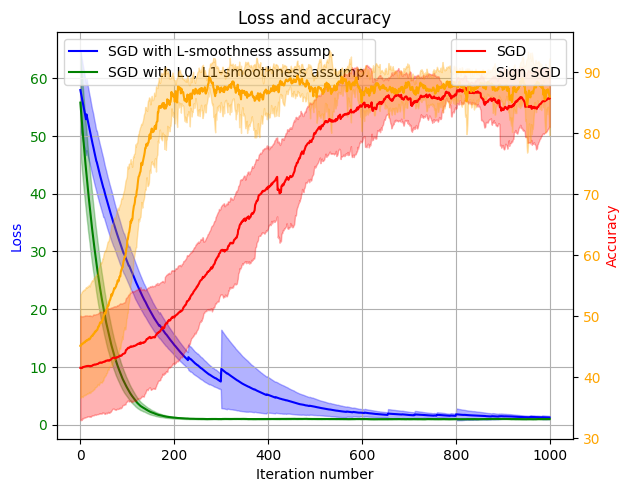
\includegraphics[width=\textwidth]{basic_experiment2.png}
        \caption{GD and SignGD with $L_1$-tuned step size.}
        \label{fig:logreg}
    \end{subfigure}
    \hfill
    \begin{subfigure}[t]{0.48\textwidth}
        \centering
        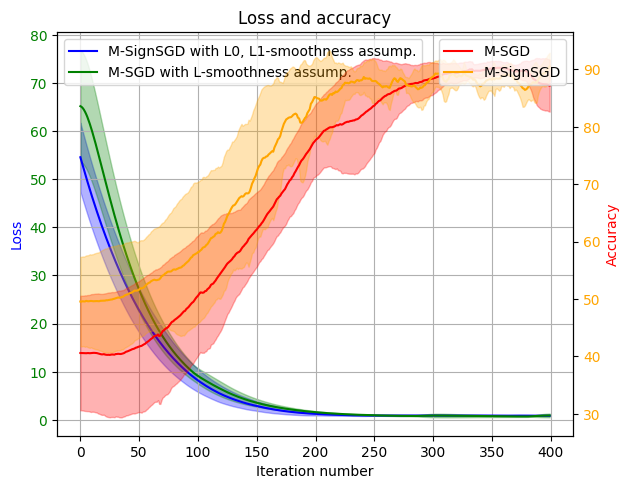
\includegraphics[width=\textwidth]{msign.png}
        \caption{ Momentum SGD  and M-SignGD with $L_1$-tuned step size.}
        \label{fig:msign}
    \end{subfigure}
    \caption{Logistic regression on Mushroom Dataset.\newline Comparison of Sign-based optimization methods.}
    \label{fig:comparison}
\end{figure}
The computational experiment aims to compare the performance of standard gradient descent (GD) and sign-based gradient descent (Sign-GD) in training a logistic regression model, highlighting the advantages of sign-based methods under $L_0, L_1$ smoothness assumptions. Performance will be evaluated based on accuracy and iteration number, with minimal tuning to emphasize simplicity.

\begin{table}[H]
\centering
\caption{Loss Comparison of Optimization Methods}
\begin{tabular}{lccc}
\toprule
\textbf{Method} & \textbf{Mean Loss} & \textbf{Loss Variance} & \textbf{Convergence Rate} \\
\midrule
M-SignSGD & 3.6366 & 73.5606 & 0.0537 \\
M-SGD     & 7.7299 & 209.4682 & 0.1289 \\
SignSGD   & 6.7171 & 155.1072 & 0.1215 \\
SGD       & 16.4469 & 234.2066 & 0.1166 \\
\bottomrule
\end{tabular}
\end{table}

\begin{table}[H]
\centering
\caption{Accuracy Comparison of Optimization Methods}
\begin{tabular}{lcc}
\toprule
\textbf{Method} & \textbf{Mean Accuracy (\%)} & \textbf{Accuracy Variance} \\
\midrule
M-SignSGD & 82.8688 & 135.7708 \\
M-SGD     & 73.4684 & 341.5860 \\
SignSGD   & 79.1219 & 140.4712 \\
SGD       & 62.9615 & 70.5549 \\
\bottomrule
\end{tabular}
\end{table}


Comments: 
The idea is based on the fact that logistic regression function $l(z,y) = \ln (1 + \exp(-yz)$  is both smooth and $(L_0, L_1)$-smooth, with $L = || y ||^2$ and $L_0 = 0, L_1 = || y ||$ which can be much smaller than $L$. Sign-GD slightly outperforms GD in accuracy and convergence time, suggesting that the sign-based update leverages smoothness assumptions effectively. The simplicity of the approach (no complex tuning) aligns with the minimal-effort goal. These results do not contradict the experiment’s aim to showcase sign-based method advantages.



\printbibliography

\newpage
\section{Proofs}

\begin{proposition}[Norm Relation]
    For two norms $ \ell_p$ and $\ell_q$ with $\ 1 \leq p \leq q \leq 2$, the following relation holds true:
    \begin{eqnarray}
        \|x\|_q \leq \|x\|_p \leq d^{\frac{1}{p} - \frac{1}{q}}\|x\|_q, \quad \forall x \in \R^d. \label{eq: norm relation}
    \end{eqnarray}
\end{proposition}

\begin{proposition}[Jensen's Inequality]
    For scalar random variable $\xi$ with bounded $\kappa$-th moment $\kappa \in (1,2]$,  the following inequality holds true:
    \begin{equation}
        \EE [|\xi|] \leq \left(\EE[|\xi|^\kappa] \right)^\frac{1}{\kappa}. \label{eq: Jensen}
    \end{equation}
\end{proposition}

\begin{proposition}[Markov's Inequality]
    For scalar random variable $\xi$ with bounded first moment, the following inequality holds true for any $a > 0$:
    \begin{equation}
        \mathbb{P}(|\xi - \EE[\xi]]| \geq a) \leq \frac{\EE[|\xi|]}{a}. \label{eq: Markov}
    \end{equation}
\end{proposition}

\begin{lemma}(Symmetric  $(L_0, L_1)$-smoothness) \label{lem: L_0,L_1 smoothness}
    Function $f:\R^d \to \R$ is asymmetrically $(L_0, L_1)$-smooth, i.e., for all $x,y \in \R^d$, it holds
    \begin{equation}
        \|\nabla f(x) - \nabla f(y)\|_2 \leq (L_0 + L_1\|\nabla f(y)\|_2)\exp(L_1\|x-y\|_2)\|x-y\|_2.
    \end{equation}
    Moreover, it implies
    \begin{eqnarray}
        f(y) \leq f(x) + \la \nabla f(x), y -x \ra + \frac{L_0 + L_1\|\nabla f(x)\|_2 }{2}\exp(L_1\|x-y\|_2)\|x-y\|_2^2.
    \end{eqnarray}
\end{lemma}

To prove the HP bounds with the logarithmic dependency, we use the following measure concentration result (see, for example, ~\cite[Lemma $1$]{li2020high}.
\begin{lemma}[Measure Concentration Lemma]\label{lem: bernstein ineq}
    Let  $\{D_k\}_{k = 1}^T$ be a martingale difference sequence (MDS), i.e., $\EE[D_k| D_{k-1}, \dots, D_1] = 0$ for all $k \in \overline{1,T}$. Furthermore, for each $k \in \overline{1,T}$, there exists positive $\sigma_k \in \R$, s.t. $\EE\left[\exp\left(\frac{D_k^2}{\sigma_k^2}\right)| k\right] \leq e.$ Then the following probability bound holds true:
    \begin{equation} \label{eq: bernstein ineq}
        \forall \lambda > 0, \delta \in (0,1): \quad \mathbb{P}\left(\sum\limits_{k=1}^T D_k \leq \frac{3}{4}\lambda \sum \limits_{k=1}^T \sigma_k^2  + \frac1\lambda \log(\nicefrac{1}{\delta})\right) \geq 1  - \delta.
    \end{equation}
\end{lemma}
To control error reduction during batching, we use the following batching lemma for HT variables. Its modern proof for $d = 1$ was proposed in ~\cite[Lemma $4.2$]{cherapanamjeri2022optimal} and then generalized for the multidimensional case  in \cite{kornilov2024accelerated, hubler2024gradient}.
\begin{lemma}[HT Batching Lemma]\label{lem: batching p}
    Let $\kappa \in (1,2]$, and $X_1, \dots, X_B \in \R^d$ be a martingale  difference sequence (MDS), i.e., $\EE[X_i| X_{i-1}, \dots, X_1] = 0$ for all $i \in \overline{1,B}$.  If all variables $X_i$ have bounded $\kappa-$th moment, i.e., $\EE[\|X_i\|_2^\kappa] < +\infty,$ then the following bound holds true
    \begin{eqnarray}
        \EE\left[\left|\left|\frac{1}{B}\sum_{i=1}^B X_i \right|\right|_2^\kappa\right]\leq \frac{2}{B^\kappa} \sum_{i=1}^B \EE[ \|X_i\|^\kappa_2]. \label{eq: HT batching}
    \end{eqnarray}
\end{lemma}
We need the following lemma about changes after one update step of sign-based methods from ~\cite[Lemma $1$]{sun2023momentum}.
\begin{lemma}[Sign Update Step Lemma] \label{lem: single update step} Let $x, m \in \R^d$ be arbitrary vectors, $A = \text{diag}(a_1, \dots, a_d)$ be diagonal matrix and $f$ be $L$-smooth function (As.~\ref{as: smooth}). Then for the update step  
$$x' = x - \gamma \cdot  A \cdot  \sign(m)$$
with $\epsilon := m - \nabla f(x)$, the following inequality holds true
\begin{equation}
    f(x') - f(x) \leq - \gamma \|A\nabla f(x)\|_1 + 2\gamma\|A\|_F\|\epsilon\|_2 + \frac{L_0 + L_1\|A  \nabla f(x^k)\|_2 }{2} \exp{(\gamma L_1\|A\|_F)}\gamma^2\|A\|^2_F . \label{eq: single sign update}
\end{equation}
\end{lemma}

\begin{proof}
    Consider the $k$-th step of \algname{SignSGD}. We use $(L_0, L_1)$ smoothness of function $f$ (Lemma \ref{lem: L_0,L_1 smoothness}) to estimate:
    \begin{eqnarray}
        f(x^{k+1}) - f(x^k) &\leq& \la \nabla f (x^k), x^{k+1} - x^k \ra + \frac{L_0 + L_1\|\nabla f(x^k)\|_2 }{2}\exp(L_1\|x^{k+1} - x^k\|_2)\|x^{k+1} - x^k\|_2^2 \notag \\
        &=& - \gamma_k  \frac{\la \nabla f (x^k), \sign(g^k) \ra}{\|\nabla f (x^k)\|_1} \cdot \|\nabla f (x^k)\|_1 + \frac{L_0d \gamma_k^2}{2}\exp(L_1\sqrt{d}\gamma_k) \notag \\ &+& \frac{ L_1d\gamma_k\exp(L_1\sqrt{d}\gamma_k) }{2}\cdot \gamma_k \|\nabla f(x^k)\|_2 \notag \\
         &\leq& - \gamma_k  \frac{\la \nabla f (x^k), \sign(g^k) \ra}{\|\nabla f (x^k)\|_1} \cdot \|\nabla f (x^k)\|_1 + \frac{L_0d \gamma_k^2}{2}\exp(L_1\sqrt{d}\gamma_k) \notag \\ &+&  \frac{ L_1d\gamma_k\exp(L_1\sqrt{d}\gamma_k) }{2}\cdot \gamma_k \|\nabla f(x^k)\|_1.\notag
    \end{eqnarray}
    Let us choose $\gamma_k \leq \frac{1}{4L_1d}$, then we have 
    $L_1d\gamma_k\exp(L_1\sqrt{d}\gamma_k) \leq \frac14$ and
    \begin{eqnarray}
        f(x^{k+1}) - f(x^k) &\leq&  - \gamma_k  \frac{\la \nabla f (x^k), \sign(g^k) \ra}{\|\nabla f (x^k)\|_1} \cdot \|\nabla f (x^k)\|_1 + L_0d \gamma_k^2 + \frac{\gamma_k}{4}  \|\nabla f(x^k)\|_1. \notag
    \end{eqnarray}

    Consequently, after summing all $T$ steps, we obtain:
    \begin{eqnarray}
        \sum \limits_{k=1}^{T} \gamma_k \left[ \frac{\la \nabla f (x^k), \sign(g^k) \ra}{\|\nabla f (x^k)\|_1} - \frac14\right] \cdot \|\nabla f (x^k)\|_1  \leq \underset{ = \Delta_1}{\underbrace{f(x^1) - f(x^*)}} + L_0d\sum \limits_{k=1}^T \gamma_k^2.
    \end{eqnarray}
    We introduce the following terms  $\phi_k := \frac{\la \nabla f (x^k), \sign(g^k) \ra}{\|\nabla f (x^k)\|_1} \in [-1,1]$, $\psi_k := \EE[\phi_k| x^{k }]$ and $D_k := - \gamma_k (\phi_k - \psi_k)\|\nabla f (x^k)\|_1$. We note that $D_k$ is a martingale difference sequence ($\EE[D_k|D_{k-1}, \dots, D_k] = 0$) and satisfies 
    $$\exp\left( \frac{D_k^2}{4\gamma_k^2\|\nabla f (x^k)\|_1^2}\right) = \exp \left(\frac{(\phi_k - \psi_k)^2}{4}\right) \leq e.$$
    Applying Measure Concentration Lemma \ref{lem: bernstein ineq} to MSD $D_k$ with $\sigma^2_k = 4 \gamma_k^2 \|\nabla f (x^k)\|_1^2$, we derive the bound for all $\lambda > 0$ with probability at least $1 - \delta$:
    $$\sum\limits_{k=1}^{T} \gamma_k(\psi_k - 3 \lambda \gamma_k \|\nabla f (x^k)\|_1 - \nicefrac{1}{4} ) \|\nabla f (x^k)\|_1 \leq \Delta_1 + L_0d\sum\limits_{k=0}^{T-1} \gamma_k^2 + \frac{1}{\lambda} \log(\nicefrac{1}{\delta}).$$
     We use norm relation \eqref{eq: norm relation} and $(L_0,L_1)$-smoothness to estimate maximum gradient norm for all $k \in \overline{2,T+1}:$
    \begin{eqnarray}
        \|\nabla f (x^k)\|_1/\sqrt{d} &\leq& \|\nabla f (x^k)\|_2 \leq \|\nabla f (x^k) - \nabla f (x^{k-1}) + \nabla f (x^{k-1}) \|_2  \notag \\
    &\leq& \|\nabla f (x^k) - \nabla f (x^{k-1})\|_2 +  \|\nabla f (x^{k-1}) \|_2 \notag \\
    &\leq&  (L_0 + L_1\|\nabla f(x^{k-1})\|_2)\exp(L_1\|x^{k} - x^{k-1}\|_2)\|x^{k} - x^{k-1}\|_2 + \|\nabla f (x^{k-1})\|_2  \notag\\
    &\leq&  (L_0 + L_1\|\nabla f(x^{k-1})\|_2)\exp(L_1\sqrt{d}\gamma_k )\sqrt{d}\gamma_k + \|\nabla f (x^{k-1})\|_2.  \notag
    \end{eqnarray}
    At this point, we take $\gamma_k \leq \frac{1}{48L_1d\log\frac1\delta \sqrt{d}}$ to obtain
    \begin{eqnarray}
        \|\nabla f (x^k)\|_1/\sqrt{d} &\leq& 2L_0\sqrt{d}\gamma_k  + \frac{\|\nabla f (x^{k-1})\|_2}{48d \log \frac1\delta}+ \|\nabla f (x^{k-1})\|_2 \notag \\
    &\leq&   2L_0\sqrt{d}\sum_{\tau=1}^{k-1}\gamma_\tau + \sum_{\tau=1}^{k-1}\frac{\|\nabla f (x^{\tau})\|_2}{48d \log \frac1\delta} + \|\nabla f (x^1)\|_2 \notag \\
    &\leq&   2L_0\sqrt{d}\sum_{\tau=1}^{k-1}\gamma_\tau + \sum_{\tau=1}^{k-1}\frac{\|\nabla f (x^{\tau})\|_1}{48d \log \frac1\delta} + \|\nabla f (x^1)\|_1. \notag
    \end{eqnarray}
    Hence, the choice $\lambda := \frac{1}{6d(\gamma^{max} \|\nabla f (x^1)\|_1  + \sum_{k=1}^{T}\frac{\gamma_k\|\nabla f (x^{k})\|_1}{48d\log \frac1\delta} + 2C_TL_0)}$ where $C_T := \max\limits_{k \in \overline{1,T}} \gamma_k \cdot  \sum\limits_{\tau=1}^{k-1}\gamma_\tau$ and $\gamma^{max} := \max\limits_{k \in \overline{1,T}} \gamma_k  $ yields with probability at least $1 - \delta$:
    \begin{eqnarray}
        \sum\limits_{k=1}^T \gamma_k\left(\psi_k - \frac{1}{2} - \frac14 \right)\|\nabla f (x^k)\|_1 &\leq& \Delta_1 + L_0d\sum_{k=1}^T\gamma_k^2 + 6\sqrt{d}(\gamma^{max} \|\nabla f (x^1)\|_1  + 2C_TL_0) \log(\nicefrac{1}{\delta}) + \notag \\ + \frac{6}{48}\sum_{k=1}^{T}\gamma_k\|\nabla f (x^{k})\|_1, \notag \\ \sum\limits_{k=1}^T \gamma_k\left(\psi_k - \frac{1}{2} - \frac14  - \frac18\right)\|\nabla f (x^k)\|_1 &\leq& \Delta_1 + L_0d\sum_{k=1}^T\gamma_k^2 + 6\sqrt{d}(\gamma^{max} \|\nabla f (x^1)\|_1  + 2C_TL_0) \log(\nicefrac{1}{\delta}), \notag \label{eq: sign sgd before prob}
    \end{eqnarray}
    Next, we estimate each term $\psi_k \|\nabla f (x^k)\|_1$ in the previous sum:
\begin{eqnarray}
\psi_k \|\nabla f (x^k)\|_1 &=& \EE \left[ \la \nabla f (x^k), \sign(g^k) \ra| x^k \right] \notag \\
&=& \|\nabla f (x^k)\|_1 - \sum_{i=1}^d 2 |\nabla f (x^k)|_i \cdot \mathbb{P}(\sign(\nabla f (x^k))_i\neq \sign(g^k)_i | x^k).\label{eq: line with prob sign}
\end{eqnarray}
For each coordinate, we have a bound derived from Markov's inequality \eqref{eq: Markov}  followed by Jensen’s inequality \eqref{eq: Jensen}:
\begin{eqnarray}
    \mathbb{P}(\sign(\nabla f (x^k))_i \neq \sign(g^k)_i | x^k) &\leq& \mathbb{P}(|\nabla f (x^k)_i -  g^k_i| \geq |\nabla f (x^k)_i| |  x^k)  
    \leq \frac{\EE_{\xi^k}[|\nabla f (x^k)_i - g^k_i| ]}{|\nabla f (x^k)_i|} \notag \\ &\leq& \frac{(\EE_{\xi^k}[|\nabla f (x^k)_i - g^k_i|^\kappa ])^\frac{1}{\kappa}}{|\nabla f (x^k)_i|}  \leq \frac{\sigma_i }{|\nabla f (x^k)_i|}. \label{eq:Prob sign not eq simple}
\end{eqnarray}
Hence, the whole sum can be bounded as 
\begin{eqnarray}
    \sum_{i=1}^d 2 |\nabla f (x^k)|_i \cdot \mathbb{P}(\sign(\nabla f (x^k))_i\neq \sign(g^k)_i | x^k)
    &\leq& 2 \|\Vec{\sigma}\|_1. \notag \notag 
\end{eqnarray}
Finally, we put this bound in \eqref{eq: sign sgd before prob} and obtain:
   \begin{eqnarray}
       \frac{1}{16} \sum\limits_{k=1}^T \gamma_k\|\nabla f (x^k)\|_1 &\leq& \Delta_1 + L_0d\sum_{k=1}^T\gamma_k^2 + 2\sum_{k=1}^T\gamma_k \|\Vec{\sigma}\|_1 \notag \\
       &+& 6d(\gamma^{max} \|\nabla f (x^1)\|_1  + 2C_TL_0) \log(\nicefrac{1}{\delta}).
   \end{eqnarray}
Plugging in constant stepsizes $\gamma_k \equiv \gamma \leq \frac{1}{48L_1d\log\frac1\delta \sqrt{d}}$ implies $C_T = T\gamma^2, \gamma^{max} = \gamma$ and the required bound:
$$\frac1T \sum\limits_{k=1}^{T} \|\nabla f (x^k)\|_1 \leq \frac{4\Delta_1}{T\gamma} + 80 L_0 d\gamma \log(\nicefrac{1}{\delta})  + 8 \|\Vec{\sigma}\|_1 + 24\frac{d\|\nabla f (x^1)\|_1}{T}  \log(\nicefrac{1}{\delta}).$$
\textbf{Case $\varepsilon \geq  \frac{8L_0}{cL_1\sqrt{d}}$:} We use stepsize $\gamma = \frac{1}{48cL_1d\log\frac1\delta \sqrt{d}} \Rightarrow 80 L_0 d\gamma \log(\nicefrac{1}{\delta}) \leq \varepsilon/2$ and  batchsize $8\frac{\|\Vec{\sigma}\|_1}{B^{\frac{\kappa-1}{\kappa}}} \leq \varepsilon/2 \Rightarrow B_k \equiv \max \left\{1,  \left(\frac{16\|\Vec{\sigma}\|_1}{\varepsilon}\right)^\frac{\kappa}{\kappa-1}\right\}$. The number of iterations  $T$ is chosen to bound the first term: 
$$\frac{4\Delta_1}{T\gamma}  = \frac{192c\Delta_1L_1\log \frac1\delta d^\frac32}{T} \leq \frac{\varepsilon}{2} \Rightarrow T = O\left(\frac{c\Delta_1 L_1  \log \frac1\delta d^\frac{3}{2}}{\varepsilon}\right).$$
The total number of oracle calls is:
\begin{eqnarray}
    \varepsilon &\geq&   \frac{8L_0}{cL_1\sqrt{d}} \quad \Rightarrow \quad N = O\left(\frac{c\Delta_1 L_1  \log(\nicefrac{1}{\delta} ) d^\frac{3}{2}}{\varepsilon}\left[1 +  \left(\frac{\|\Vec{\sigma}\|_1}{\varepsilon}\right)^\frac{\kappa}{\kappa-1}\right]\right), \notag 
\end{eqnarray}
\textbf{Case $\varepsilon < \frac{8L_0}{L_1\sqrt{d}}$:} We set the same batchsize $8\frac{\|\Vec{\sigma}\|_1}{B^{\frac{\kappa-1}{\kappa}}} \leq \varepsilon/2 \Rightarrow B_k \equiv \max \left\{1,  \left(\frac{16\|\Vec{\sigma}\|_1}{\varepsilon}\right)^\frac{\kappa}{\kappa-1}\right\}$. The stepsize $\gamma$ is set to minimize the sum:
$$\min_\gamma \left[ \frac{4\Delta_1}{T\gamma} + 80 L_0 d\gamma \log(\nicefrac{1}{\delta}) \right] = 2\sqrt{\frac{320\Delta_1 L_0 d \log(\nicefrac{1}{\delta})}{T}} ,$$
it means that the stepsize $\gamma = \sqrt{\frac{4\Delta_1}{80 TL_0\log(\nicefrac{1}{\delta})d}}$. The number of iterations $T$ is chosen to satisfy $$2\sqrt{\frac{320\Delta_1 L_0  \log(\nicefrac{1}{\delta})d}{T}} \leq \frac{\varepsilon}{2} \Rightarrow T = O \left(\frac{\Delta_1 L_0  \log(\nicefrac{1}{\delta})d}{\varepsilon^2}\right).$$
We only need to check whether condition $\gamma \leq \frac{1}{48L_1d\log\frac1\delta \sqrt{d}}$ holds:
\begin{eqnarray}
    \gamma &=& \sqrt{\frac{4\Delta_1}{80 TL_0\log(\nicefrac{1}{\delta})d}} = \sqrt{\frac{4\Delta_1}{ T} \frac{1}{80L_0\log(\nicefrac{1}{\delta})d}} \notag \\
    &\leq& \frac{\varepsilon}{4} \frac{1}{80L_0\log(\nicefrac{1}{\delta})d} \leq \frac{8L_0}{4L_1 \sqrt{d}} \frac{1}{80L_0\log(\nicefrac{1}{\delta})d} \notag \\
    &\leq& \frac{1}{48L_1d\log\frac1\delta \sqrt{d}}. \notag
\end{eqnarray}
Hence, we have the following bound for sample complexity
\begin{eqnarray}
\varepsilon &<& \frac{8L_0}{L_1\sqrt{d}} \quad \Rightarrow \quad N = O\left(\frac{\Delta_1L_0\log(\nicefrac{1}{\delta} ) d }{\varepsilon^2}\left[1 +  \left(\frac{\|\Vec{\sigma}\|_1}{\varepsilon}\right)^\frac{\kappa}{\kappa-1}\right]\right). 
\end{eqnarray}
\end{proof}


\subsection{Proof of Sign Update Step Lemma}  
\begin{proof} 
The proof is identical to the proof from ~\cite[Lemma $1$]{sun2023momentum} with changing the smoothness assumption according to Lemma \ref{lem: L_0,L_1 smoothness}.
Using the $(L_0, L_1)$-smoothness of $f$, we have
\[
f(x') \leq f(x) + \langle \nabla f(x), x' - x \rangle + \frac{L_0 + L_1\|x' - x\|}{2} \|x' - x\|^2 \exp(L_1\|x' - x\|).
\]
Substitute $x' - x = -\gamma A \sign(m)$:
\[
\langle \nabla f(x), x' - x \rangle = -\gamma \langle \nabla f(x), A \sign(m) \rangle.
\]

We now decompose the inner product:
\[
\langle \nabla f(x), A \sign(m) \rangle = \langle \nabla f(x), A \sign(\nabla f(x)) \rangle + \langle \nabla f(x), A(\sign(m) - \sign(\nabla f(x))) \rangle.
\]

Using the identity:
\[
\langle \nabla f(x), A \sign(\nabla f(x)) \rangle = \|A \nabla f(x)\|_1,
\]
and define $[\nabla f(x)]_i =: g_i$, then the second term becomes
\[
\sum_{i=1}^d a_i g_i \left( \sign(m_i) - \sign(g_i) \right).
\]

Now we analyze two cases for each $i$:
\begin{itemize}
    \item If $\sign(m_i) = \sign(g_i)$, then the term is zero.
    \item Otherwise, $g_i \cdot m_i \leq 0$, hence $|g_i - m_i| \geq |g_i|$, and we define $\epsilon_i = m_i - g_i$. Then:
    \[
    a_i g_i \left( \sign(m_i) - \sign(g_i) \right) \leq 2a_i |g_i| \leq 2a_i |\epsilon_i|.
    \]
\end{itemize}

So we have:
\[
\langle \nabla f(x), A \sign(\nabla f(x)) - A \sign(m) \rangle \leq  2 \sum_{i=1}^d a_i |\epsilon_i| \leq  2\|A\|_F\|\epsilon\|_2.
\]

Thus,
\[
\langle \nabla f(x), x' - x \rangle \leq -\gamma \|A \nabla f(x)\|_1 + 2\gamma \|A\|_F \|\epsilon\|_2.
\]

Now, observe that
\[
\|x' - x\| = \gamma \|A \sign(m)\|_2 \leq \gamma \|A\|_F.
\]

Substituting into the smoothness upper bound:
\[
f(x') - f(x) \leq -\gamma \|A \nabla f(x)\|_1 + 2\gamma \|A\|_F \|\epsilon\|_2 + \frac{L_0 + L_1\|A \nabla f(x)\|_2}{2} \exp(\gamma L_1 \|A\|_F) \gamma^2 \|A\|_F^2.
\]
\end{proof}

\subsection{Proof of $(L_0,L_1)$ \algname{M-SignSGD} General Convergence }  
\begin{proof}

    Consider the $k$-th step of \algname{SignSGD}. We use $(L_0, L_1)$ step update (Lemma \ref{lem: single update step}) to estimate:
    \begin{eqnarray}
        f(x^{k+1}) - f(x^k) &\leq& \la \nabla f (x^k), x^{k+1} - x^k \ra + \frac{L_0 + L_1\|\nabla f(x^k)\|_2 }{2}\exp(L_1\|x^{k+1} - x^k\|_2)\|x^{k+1} - x^k\|_2^2 \notag \\ &\leq&  - \gamma_k\| \nabla f (x^k)\|_1 + 2\gamma_k \sqrt{d} \| \epsilon^k\|_2 + \frac{L_0d \gamma_k^2}{2}\exp(L_1\sqrt{d}\gamma_k) \notag \\ &+&  \frac{ L_1d \gamma_k\exp(L_1\sqrt{d}\gamma_k) }{2}\cdot \gamma_k \|\nabla f(x^k)\|_1.\notag  
    \end{eqnarray}
    
The inequality holds due to Lemma \ref{lem: single update step}.

Since we set constant steps sizes and momentum, we denote them as $\gamma \equiv \gamma_k$ and $\beta \equiv \beta_k$, respectively. We use notations $\epsilon^k := m^k - \nabla f(x^k)$ and $\theta^k := g^k - \nabla f(x^k)$. Therefore, we have at $k$-th step values:
\begin{eqnarray}
    m^k &=& \beta m^{k-1} + (1-\beta) g^k= \gamma (\epsilon^{k-1} + \nabla f(x^{k-1})) + (1-\gamma)(\theta^k + \nabla f(x^k)),\notag \\
    \epsilon^k &=& m^k - \nabla f(x^k) = \beta \epsilon^{k-1} + \beta(\underset{=:s^k}{\underbrace{\nabla f (x^{k-1}) - \nabla f (x^k)}} ) + (1- \beta)\theta^k, \notag\\
    \epsilon^k &=& m^k - \nabla f(x^k) = \beta \epsilon^{k-1} + \beta s^k + (1- \beta)\theta^k.\notag 
\end{eqnarray}
Unrolling the recursion, we obtain an explicit formula (upper index of $\beta$ is its power):
\begin{eqnarray}
\epsilon^{k} &=& \beta^{k-1}\epsilon^1 + \sum_{i=2}^{k} \beta^{k-i + 1} s^i + (1-\beta) \sum_{i=2}^{k} \beta^{k-i} \theta^i. \label{eq: unrolling m-signsgd}
\end{eqnarray}

From $(L_0, L_1)-$smoothness of $f$ (Lem. \ref{lem: L_0,L_1 smoothness}) follows the bound:
$$\|s^k\|_2 \leq (L_0 + L_1\|\nabla f(x^k)\|_2)\exp(L_1\|x^k-x^{x + 1}\|_2)\|x^k-x^{k + 1}\|_2 = (L_0 + L_1\|\nabla f(x^k)\|_2)\exp(L_1\gamma_k\sqrt{d})\gamma_k\sqrt{d} $$
Denote $\lambda := \exp(L_1\gamma_k\sqrt{d})\gamma_k\sqrt{d}$.

Hence, the norm of \eqref{eq: unrolling m-signsgd} can be bounded as:
$$\|\epsilon^k\|_2 \leq \beta^{k-1}\|\epsilon^1\|_2 + L_0\lambda \sum_{i=2}^{k} \beta^{k-i + 1} + L_1\lambda \sum_{i=2}^{k}\beta^{k-i + 1}  \|\nabla f(x^k)\|_2+ (1-\beta) \|\sum_{i=2}^k \beta^{k-i} \theta^i\|_2.$$
We notice that variables $\{\theta_i\}$ are martingale difference sequence from Lemma \ref{lem: batching p} which we plan to use. Due to the formal definition of $\theta^i = g^i - \nabla f(x^i) = \nabla f(x^i, \xi_i) - \nabla f(x^i)$ and \algname{M-SinSGD} step, the conditioning on $ \theta^{i-1}, \dots, \theta^1$  with randomness $\xi_1, \dots, \xi_{i-1} $ is equivalent to the conditioning on point s $x^{i},\dots ,x^{2}$. Hence, we show by definition of martingale difference sequence that  $$\EE[\theta^i| \theta^{i-1}, \dots, \theta^1 ] = \EE[\theta^i|x^{i},\dots ,x^{2}] = \EE[\nabla f(x^i, \xi_i) - \nabla f(x^i)|x^{i},\dots ,x^{2}] = 0.$$

To take math expectation from both sides, we first take it from the term
\begin{eqnarray}
    \EE \left[ \|\sum_{i=2}^k \beta^{k-i} \theta^i\|_2 \right]\leq \left(\EE \left[\|\sum_{i=2}^k \beta^{k-i} \theta^i\|_2^\kappa\right]\right)^\frac1\kappa \overset{\text{Lem. }\ref{lem: batching p} }{\leq} \left(\sum_{i=2}^k 2 \EE \left[\| \beta^{(k-i)}\theta^i\|_2^\kappa\right]\right)^\frac1\kappa \leq  \left(\sum_{i=2}^k 2 \beta^{\kappa(k-i)}\EE \left[\| \theta^i\|_2^\kappa\right]\right)^\frac1\kappa. \notag \label{eq: m-signsgd 1} %\leq \frac{2\|\Vec{\sigma}\|_\kappa}{(1 - \beta^\kappa)^\frac1\kappa}.
\end{eqnarray}
For each $i \in \overline{2,T}$, we estimate $\EE \left[\| \theta^i\|_2^\kappa\right]$ as 
\begin{eqnarray}
    \EE \left[\| \theta^i\|_2^\kappa\right] \overset{\eqref{eq: norm relation}}{\leq } \EE \left[\| \theta^i\|_\kappa^\kappa\right] = \EE \left[\sum_{j=1}^d| g^k_j - \nabla f(x^k)_j|^\kappa\right] \overset{As. \ref{as: pBCM}}{\leq }  \sum_{j=1}^d \sigma^\kappa_j = \|\Vec{\sigma}\|_\kappa^\kappa. 
\end{eqnarray}
We continue bounding \eqref{eq: m-signsgd 1} with
\begin{eqnarray}
    \eqref{eq: m-signsgd 1} \leq \left(\sum_{i=2}^k 2 \beta^{\kappa(k-i)}\|\Vec{\sigma}\|_\kappa^\kappa\right)^\frac1\kappa \leq \frac{2\|\Vec{\sigma}\|_\kappa}{(1 - \beta^\kappa)^\frac1\kappa}. \notag
\end{eqnarray}
Therefore, the final math expectation can be calculated as:
\begin{eqnarray}
     \EE\|\epsilon^k\|_2 &\leq& \beta^{k-1} \EE \|\epsilon^1\|_2 + \frac{L\sqrt{d}\gamma}{1 - \beta}   + \frac{2(1-\beta) \|\Vec{\sigma}\|_\kappa}{(1 - \beta^\kappa)^\frac1\kappa}.
\end{eqnarray}



%% =================================== {\color{red} add terms}


Now, we can update the step using Lemma \ref{lem: single update step}:
\begin{eqnarray} 
\end{eqnarray}
Then take math expectation:
\begin{eqnarray}
    f(x^{k+1}) - f(x^k) &\leq&  - \gamma \| \nabla f (x^k)\|_1 + 2\gamma \sqrt{d} \| \epsilon\|_2 + \frac{L_0\sqrt{d} \gamma}{2}\lambda \notag  + \frac{ L_1 \sqrt{d} \gamma_k }{2}\cdot \lambda \|\nabla f(x^k)\|_1\\ &\leq&  - \gamma\| \nabla f(x^k)\|_1 \notag  + 2\gamma \sqrt{d}\cdot\\ &+&  \left[ \beta^{k-1}\|\epsilon^1\|_2 + L_0\lambda \sum_{i=2}^{k} \beta^{k-i + 1} + L_1\lambda \sum_{i=2}^{k}\beta^{k-i + 1}  \|\nabla f(x^i)\| +  (1-\beta) \|\sum_{i=2}^k \beta^{k-i} \theta^i\|_2\right] \notag  \\&+&\frac{L_0\sqrt{d} \gamma}{2}\lambda \notag  + \frac{ L_1 \sqrt{d} \gamma }{2}\cdot \lambda \|\nabla f(x^k)\|_1 \\&\leq&  - \gamma\| \nabla f(x^k)\|_1 \notag \\&+&  2\gamma \sqrt{d}\left[ \beta^{k-1}\|\epsilon^1\|_2 + L_0\lambda \frac{1}{1 - \beta} + L_1\lambda \sum_{i=2}^{k}\beta^{k-i + 1} \|\nabla f(x^i)\| +  (1-\beta) \|\sum_{i=2}^k \beta^{k-i} \theta^i\|_2\right] \notag  \\&+&\frac{L_0\sqrt{d} \gamma}{2}\lambda \notag  + \frac{ L_1 \sqrt{d} \gamma }{2}\cdot \lambda \|\nabla f(x^k)\|_1 \notag
\end{eqnarray}
\begin{eqnarray}
   \EE[f(x^{k+1})] - \EE[f(x^k)] &\leq& - \gamma \EE[\|\nabla f(x^k)\|_1] + 2\gamma \sqrt{d} \beta^{k-1} \EE \|\epsilon^1\|_2\\ &+& \notag L_0\lambda \frac{2\gamma \sqrt{d}}{1 - \beta} + L_1\lambda 2\gamma \sqrt{d} \sum_{i=2}^{k}\beta^{k-i + 1} \EE \|\nabla f(x^k)\|_1 + \frac{4\gamma \sqrt{d}(1-\beta) \|\Vec{\sigma}\|_\kappa}{(1 - \beta^\kappa)^\frac1\kappa} \notag \\&+& \frac{L_0\sqrt{d} \gamma}{2}\lambda \notag  + \frac{ L_1 \sqrt{d} \gamma }{2}\lambda \EE \|\nabla f(x^k)\|_1 \notag 
\end{eqnarray}
Summing it over $k$, we derive

\begin{eqnarray}
   f^* - f(x^1)&\leq& - \gamma \sum_{k=1}^T\EE\|\nabla f(x^k)\|_1 + 2\gamma T \sqrt{d} \beta^{k-1} \EE \|\epsilon^1\|_2\\\notag  &+& \notag  L_1\lambda 2\gamma \sqrt{d}  \sum_{k=1}^T\sum_{i=2}^{k}\beta^{k-i + 1} \EE \|\nabla f(x^i)\|_1 + \frac{4\gamma T \sqrt{d}(1-\beta) \|\Vec{\sigma}\|_\kappa}{(1 - \beta^\kappa)^\frac1\kappa} \notag \\&+& \frac{L_0 T \sqrt{d} \gamma}{2}\lambda \notag  + \frac{ L_1 \sqrt{d} \gamma }{2}\lambda \sum_{k=1}^T \EE \|\nabla f(x^k)\|_1 \notag
   \label{eq: m-signsgd prefinal}
\end{eqnarray}

Changing the order of summation in the right part of the  \eqref{eq: m-signsgd prefinal} we obtain:

\begin{eqnarray} 
2\gamma L_1\lambda \sqrt{d} \sum_{k=1}^T  
 \left( \sum_{i=2}^{k}\beta^{k-i + 1} \EE \|\nabla f(x^i)\|_1 \right) \notag \notag  &=& \\  2\gamma L_1\lambda \sqrt{d}  \sum_{i=2}^T\left( \sum_{k = i}^{T}\beta^{k-i + 1} \EE \|\nabla f(x^i)\|_1 \right) &=& \notag \\  2\gamma L_1\lambda \sqrt{d}  \sum_{i=2}^T \beta^{-i} \left( \sum_{k = i}^{T}\beta^{k + 1} \right) \EE \|\nabla f(x^i)\|_1 &=& \notag \\ 2\gamma L_1\lambda \sqrt{d}  \sum_{i=2}^T \beta^{-i + 1} \beta^i \left(\frac{1 - \beta^{T - i}}{1 - \beta} \right) \EE \|\nabla f(x^i)\|_1 \notag  &\leq& \\  2\gamma L_1\lambda \sqrt{d}  \sum_{i=2}^T  \beta \left(\frac{1}{1 - \beta} \right) \EE \|\nabla f(x^i)\|_1 \notag  
    \label{eq: m-signsgd 2} 
\end{eqnarray}

Finally 
\begin{eqnarray}
   f^* - f(x^1)  &\leq&  - \gamma \sum_{k=1}^T\EE\|\nabla f(x^k)\|_1 + \frac{2\gamma \sqrt{d} \EE \|\epsilon^1\|_2}{1 - \beta}\\ &+& 2\gamma L_1\lambda \sqrt{d} \cdot \frac{\beta}{1 - \beta} \sum_{k = 1}^T \EE \|\nabla f(x^k)\|_1 \notag + \frac{4\gamma T \sqrt{d}(1-\beta)\|\Vec{\sigma}\|_\kappa}{(1 - \beta^\kappa)^{1/\kappa}} \\ &+& \frac{L_0 T \sqrt{d} \gamma}{2 (1 - \beta)}\lambda + \frac{L_1 \sqrt{d} \gamma}{2}\lambda \sum_{k=1}^T \EE \|\nabla f(x^k)\|_1 \notag 
 \\ &\leq&  \left(- \gamma +  \frac{2\gamma L_1\lambda \sqrt{d}\beta}{1 - \beta} +\frac{L_1 \sqrt{d} \gamma}{2}\lambda  \right) \sum_{k=1}^T\EE\|\nabla f(x^k)\|_1 \\ &+&  \notag \frac{2\gamma \sqrt{d} \EE \|\epsilon^1\|_2}{1 - \beta} + \frac{4\gamma T \sqrt{d}(1-\beta)\|\Vec{\sigma}\|_\kappa}{(1 - \beta^\kappa)^{1/\kappa}} + \frac{L_0 T \sqrt{d} \gamma}{2 (1 - \beta)}\lambda.
 \label{eq: m-signsgd final} 
\end{eqnarray}
Let us set stepsize $\gamma$ such that 
$$\frac{2\gamma L_1\lambda \sqrt{d}\beta}{1 - \beta} +\frac{L_1 \sqrt{d} \gamma}{2}\lambda \leq \frac{3\gamma^2 L_1 d \exp(L_1 d \gamma)}{1 - \beta}  \leq \gamma/2 \Rightarrow\gamma \leq \frac{1 - \beta}{8} \frac{1}{L_1d}. $$
Thus, we obtain
\begin{eqnarray}
    f^* - f(x^1)  &\leq&  -\frac{\gamma}{2} \sum_{k=1}^T\EE\|\nabla f(x^k)\|_1 + \frac{2\gamma \sqrt{d} \EE \|\epsilon^1\|_2}{1 - \beta} + 4\gamma T \sqrt{d}(1-\beta)^\frac{\kappa - 1}{\kappa}\|\Vec{\sigma}\|_\kappa + \frac{L_0 T d \gamma^2}{(1 - \beta)}, \notag \\
    \frac{1}{T} \sum_{k=1}^T\EE\|\nabla f(x^k)\|_1 &\leq& \frac{2(f^* - f(x^1))}{\gamma T} + \frac{4 \sqrt{d}  \EE \|\epsilon^1\|_2}{T(1 - \beta)} + 8 \sqrt{d}(1-\beta)^\frac{\kappa - 1}{\kappa}\|\Vec{\sigma}\|_\kappa + \frac{2L_0 d \gamma}{(1 - \beta)}.
\end{eqnarray}
\textbf{Case $\varepsilon \geq \frac{3L_0}{L_1 c}$.} 
We choose the stepsize $\gamma  = \frac{1 - \beta}{8} \frac{1}{L_1dc} \leq \frac{1 - \beta}{8} \frac{1}{L_1d}$ and get:
\begin{eqnarray}
    \frac{1}{T} \sum_{k=1}^T\EE\|\nabla f(x^k)\|_1 &\leq& \frac{16c\Delta_1 L_1 d}{T(1 - \beta)} + \frac{4 \sqrt{d}  \EE \|\epsilon^1\|_2}{T(1 - \beta)} + 8 \sqrt{d}(1-\beta)^\frac{\kappa - 1}{\kappa}\|\Vec{\sigma}\|_\kappa + \frac{4L_0}{L_1c} \notag \\
    &\leq& \frac{16c(\Delta_1 L_1 + \EE \|\epsilon^1\|_2) d}{T(1 - \beta)}+ 8 \sqrt{d}(1-\beta)^\frac{\kappa - 1}{\kappa}\|\Vec{\sigma}\|_\kappa + \frac{4\varepsilon}{3}. \notag
\end{eqnarray}
Then, we  choose $1 - \beta = \min\left\{1, \left(\frac{c\Delta_1 L_1 \sqrt{d}}{T \|\Vec{\sigma}\|_\kappa}\right)^\frac{\kappa}{2\kappa - 1}\right\}$ to obtain
\begin{eqnarray}
    \min_{\beta \in [0,1)} \left[ \frac{16c\Delta_1 L_1 d}{T(1 - \beta)}+ 8 \sqrt{d}(1-\beta)^\frac{\kappa - 1}{\kappa}\|\Vec{\sigma}\|_\kappa \right] \leq 24\sqrt{d} \left( \frac{c\Delta_1 L_1 \sqrt{d}}{T}\right)^\frac{\kappa - 1}{2\kappa - 1}\|\Vec{\sigma}\|_\kappa^\frac{\kappa}{2\kappa - 1} + \frac{24c\Delta_1 L_1 d}{T}.
\end{eqnarray}
Finally, we choose number of iterations $T$ to get:
$$24\sqrt{d} \left( \frac{c\Delta_1 L_1 \sqrt{d}}{T}\right)^\frac{\kappa - 1}{2\kappa - 1}\|\Vec{\sigma}\|_\kappa^\frac{\kappa}{2\kappa - 1} + \frac{24c\Delta_1 L_1 d}{T} \leq \varepsilon  \Rightarrow T = O\left(\frac{c\Delta_1L_1d}{\varepsilon } \left(1 + \left(\frac{\sqrt{d}\|\Vec{\sigma}\|_\kappa}{\varepsilon}\right)^\frac{\kappa }{\kappa  -1}\right)\right).$$


\textbf{Case $\varepsilon \leq \frac{3L_0}{L_1}$.} We choose stepsize $\gamma = \sqrt{\frac{\Delta_1 (1 - \beta)}{T L_0 d}}$ to minimize the sum
\begin{eqnarray}
    \min_\gamma \left[\frac{2(f^* - f(x^1))}{\gamma T} + \frac{2L_0 d \gamma}{(1 - \beta)} \right] = 4\sqrt{\frac{\Delta_1 L_0 d}{T(1-\beta)}}, \notag
\end{eqnarray}
\begin{eqnarray}
    \frac{1}{T} \sum_{k=1}^T\EE\|\nabla f(x^k)\|_1 &\leq&  \frac{4 \sqrt{d}  \EE \|\epsilon^1\|_2}{T(1 - \beta)} + 4\sqrt{\frac{\Delta_1 L_0 d}{T(1-\beta)}} + 8 \sqrt{d}(1-\beta)^\frac{\kappa - 1}{\kappa}\|\Vec{\sigma}\|_\kappa.
\end{eqnarray}
The first term is much smaller than the second one, hence we omit it. Next, we choose $1  - \beta =   \min\left\{1, \left(\frac{\Delta_1 L_0}{T \|\Vec{\sigma}\|_\kappa^2}\right)^\frac{\kappa}{3\kappa - 2}  \right\}$ to minimize the last two terms:
$$\min_{\beta \in [0,1)} \left[ 4\sqrt{\frac{\Delta_1 L_0 d}{T(1-\beta)}} + 8 \sqrt{d}(1-\beta)^\frac{\kappa - 1}{\kappa}\|\Vec{\sigma}\|_\kappa \right] \leq 12 \sqrt{d} \left(\frac{\Delta_1L_0}{T}\right)^\frac{\kappa - 1}{3\kappa - 2} \|\Vec{\sigma}\|_\kappa^\frac{\kappa}{3\kappa  - 2} + 12 \sqrt{\frac{\Delta_1 L_0 d}{T}}.$$
Finally, we choose number of iterations $T$ to satisfy:
\begin{eqnarray}
    12 \sqrt{d} \left(\frac{\Delta_1L_0}{T}\right)^\frac{\kappa - 1}{3\kappa - 2} \|\Vec{\sigma}\|_\kappa^\frac{\kappa}{3\kappa  - 2}  + 12 \sqrt{\frac{\Delta_1 L_0 d}{T}}\leq \frac{\varepsilon}{2} \Rightarrow T = O\left(\frac{\Delta_1L_0d}{\varepsilon^2 } \left( 1 + \left(\frac{\sqrt{d}\|\Vec{\sigma}\|_\kappa}{\varepsilon}\right)^\frac{\kappa }{\kappa  -1}\right)\right).
\end{eqnarray}
We only need to check that
$$\gamma = \sqrt{\frac{\Delta_1 (1 - \beta)}{T L_0 d}} = \sqrt{\frac{\Delta_1 L_0 d}{T (1-\beta)}} \frac{(1-\beta)}{L_0 d}  \leq \frac{\varepsilon}{2 \cdot 12} \frac{(1-\beta)}{L_0 d} \overset{\varepsilon \leq \frac{3L_0}{L_1}}{\leq} \frac{(1-\beta)}{L_1 d}.$$
 \end{proof}

\newpage

 
\end{document}


\printbibliography

\end{document}
